\section{Implementation}
\subsection{Parallel radix-$2^3$ 16-Points}
\begin{frame}
  \frametitle{\textbf{Table of Contents}}
  \begin{center}
    {\vspace{-1.5cm}\Large \textbf{Section \thesection}\vspace{0.5cm}}
    \begin{beamercolorbox}[
      sep=8pt,center]{part title}
      \usebeamerfont{part title}
      \textbf{\insertsection}
    \end{beamercolorbox}
  \end{center}
\end{frame}


\subsection{Floating and Fixed point Simulator}


\begin{frame}
	\frametitle{\textbf{Design of FFT architecture via folding transformation}}
	\framesubtitle{\secname : \subsecname}
	\begin{block}{\centering \textbf{Signal Quantization}}
		\begin{itemize}\justifying\footnotesize
        	\item The signals in each stage are quantized in order to obtain a high SQNR\footnote{Signal to Quantization Noise Ratio}($\approx 50\, dB$).
			\begin{equation*}%\label{eq:sqnr}
			SQNR_{dB} = 10log_{10} \bigg(  \frac{  Var\{Signal_{FloatPoint}\}  }{  Var\{Signal_{FloatPoint} - Signal_{FixedPoint}\}}  \bigg)
			\end{equation*}
			\item The quantization of the signals is:
			\begin{itemize}\justifying\footnotesize
				\item Input: $S(10,9)$, $SQNR \approx 57\,dB$.
				\item Twiddle factors: $S(11,9)$.
				\item Output: $S(22,15)$, $SQNR \approx 47\,dB$.				
			\end{itemize}			 
		\end{itemize}	
	\end{block}
\end{frame}



\begin{frame}
	\frametitle{\textbf{Design of FFT architecture via folding transformation}}
	\framesubtitle{\secname : \subsecname}
	\begin{block}{\centering \textbf{Testing signals}}
		\begin{itemize}\justifying\footnotesize
        	\item The input signal will be a mixture of two sinusoid signals with frecuencies  $f_1=100Hz$, $f_2=1000Hz$.
        	%\item This signal will be noramalized to the unity.
		\begin{align}\label{eq: inputSignal}
			x'[n] &= cos(2\pi f_1 n T_s) + cos(2\pi f_2 n T_s)  \\
			x[n] &= x'[n]/max\{x'[n]\} 						\nonumber
		\end{align}
		\end{itemize}	
	\end{block}
	\vspace{-0.75cm}
	\begin{columns}[t,onlytextwidth]
		\begin{column}{0.45\linewidth}
   			\begin{figure}[h!] \centering
	    		\includegraphics[height=0.35\paperheight]{./image/input_fx.pdf}
				\caption{\tiny Input signal $x[n]$ in time domain.}
	    	\end{figure}
	    \end{column}
	    \begin{column}{0.45\linewidth}
	    	\begin{figure}[h!] \centering
	    		\includegraphics[height=0.35\paperheight]{./image/output_fx.pdf}
				\caption{\tiny Output samples, absolute value vs frequency $|X[k]|$.}
	    	\end{figure}  
   		\end{column}
	\end{columns}  
\end{frame}


\begin{frame}
	\frametitle{\textbf{Design of FFT architecture via folding transformation}}
	\framesubtitle{\secname : \subsecname}
	\begin{block}{\centering \textbf{Design Implementations}}
		\begin{itemize}\justifying\footnotesize
        	\item Design 1: 
        	\begin{itemize}\justifying\footnotesize
        		\item Quantitions blocks placed after the multiplers in each stage.
        		\item Multiplicators are not optimized.
			\end{itemize}        		 
        	\item Design 2:
			\begin{itemize}\justifying\footnotesize
				\item  A Pipeline cut-set is added after every quantization block.
			\end{itemize}				        	
        	\item Design 3:
        	\begin{itemize}\justifying\footnotesize
     			\item Implementation with Trival multiplicators for $-j$ factors. 
			\end{itemize}
        	\item Design 4:
        	\begin{itemize}\justifying\footnotesize
				\item A Pipeline cut-set is added inside of each butterfly block.				
				\item  Implementation of CSD multipliers.
			\end{itemize}
		\end{itemize}        	
	\end{block}
\end{frame}



\begin{frame}
	\frametitle{\textbf{Design of FFT architecture via folding transformation}}
	\framesubtitle{\secname : \subsecname}
	\vspace{-0.5cm}
		\begin{figure}[h!] \centering
		   	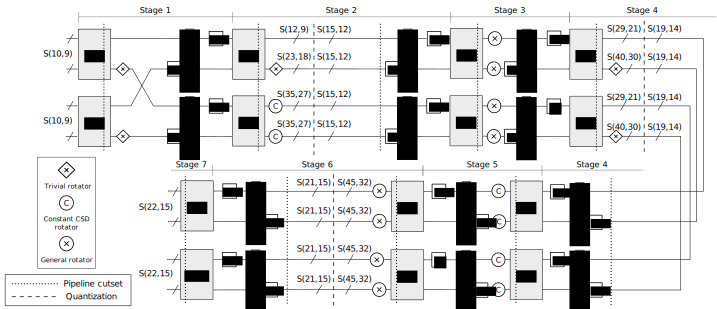
\includegraphics[width=0.95\paperwidth]{./image/folding-128-quant.pdf}
		   	\caption{ \tiny Folding architecture for radix-$2^3$  128 points FFT with quatization (Design 1).}
		\end{figure}  	
\end{frame}


\begin{frame}
	\frametitle{\textbf{Design of FFT architecture via folding transformation}}
	\framesubtitle{\secname : \subsecname}
	\vspace{-0.5cm}	
		\begin{figure}[h!] \centering
		   	\includegraphics[width=0.95\paperwidth]{./image/folding-128-quant-pipe.png}
		   	\caption{ \tiny Folding architecture for radix-$2^3$ 128 points FFT with quantization and pipeline (Design 4).}
		\end{figure}  	
\end{frame}



\subsection{Results}

\begin{frame}
	\frametitle{\textbf{Design of FFT architecture via folding transformation}}
	\framesubtitle{\secname : \subsecname}
	\centering\textbf{Timing Report at 500MHz}
	\vspace{-0.75cm}
	\begin{columns}[t,onlytextwidth]
		\begin{column}{0.45\linewidth}
		   \begin{table}[t!]
			\centering%\raggedleft%\flushright 	
			\resizebox{0.6\linewidth}{!}{%			
			\begin{tabular}{@{}lr@{}}
				%\hline\hline
				Point 						& Path(ns)\\
				\hline\hline
				data arrival time   		& 5.60\\ 
				clock CLK (rise edge)  		& 2.00\\
				clock network delay (ideal) & 2.00\\
				library setup time			& 1.95\\
				\hline
				data required time			& 1.95\\
				data arrival time           & -5.60\\
				\hline
				slack (VIOLATED)            & -3.65\\	
				\hline
			\end{tabular}}
			\caption{\footnotesize Design instance 1.}			
			\end{table}
			%
			\vspace{-0.75cm}
			\begin{table}[t!]
			\centering%\raggedleft%\flushright 	
			\resizebox{0.6\linewidth}{!}{%
			\begin{tabular}{@{}lr@{}}
				%\hline\hline
				Point 						&Path(ns)\\
				\hline\hline
				data arrival time   		&2.76\\ 
				clock CLK (rise edge)  		&2.00\\
				clock network delay (ideal) &2.00\\
				library setup time			&1.95\\
				\hline
				data required time			&1.95\\
				data arrival time           &-2.76\\
				\hline
				slack (VIOLATED)            &-0.81\\	
				\hline
			\end{tabular}}
			\caption{\footnotesize Design instance 3.}
			\end{table}
   		\end{column}
   		%
		\begin{column}{0.45\linewidth}
			\begin{table}[t!]
			\centering%\raggedleft%\flushright 	
			\resizebox{0.6\linewidth}{!}{%			
				\begin{tabular}{@{}lr@{}}
				%\hline\hline
				Point 						&Path(ns)\\
				\hline\hline
				data arrival time   		&2.71\\ 
				clock CLK (rise edge)  		&2.00\\
				clock network delay (ideal) &2.00\\
				library setup time			&1.95\\
				\hline
				data required time			&1.95\\
				data arrival time           &-2.71\\
				\hline
				slack (VIOLATED)            &-0.76\\	
				\hline
			\end{tabular}}
			\caption{\footnotesize Design instance 2.}
			\end{table}
			\vspace{-0.75cm}
			\begin{table}[t!]
			\centering%\raggedleft%\flushright 	
			\resizebox{0.6\linewidth}{!}{%
			\begin{tabular}{@{}lr@{}}
				%\hline\hline
				Point 						& Path(ns)\\
				\hline\hline
				data arrival time   		&1.94\\ 
				clock CLK (rise edge)  		&2.00\\
				clock network delay (ideal) &2.00\\
				library setup time			&1.94\\
				\hline
				data required time			&1.94\\
				data arrival time           &-1.94\\
				\hline
				slack (MET)                 &0.00\\	
				\hline
			\end{tabular}}
			\caption{\footnotesize Design instance 4.}			
			\end{table}
   		\end{column}   		
	\end{columns}  
\end{frame}


\begin{frame}
	\frametitle{\textbf{Design of FFT architecture via folding transformation}}
	\framesubtitle{\secname : \subsecname}
	\centering\textbf{Area Report at 500MHz}
	\vspace{-1cm}
	\begin{columns}[t,onlytextwidth]
		\begin{column}{0.45\linewidth}
		   \begin{table}[t!]
			\centering%\raggedleft%\flushright 	
			\resizebox{0.65\linewidth}{!}{%			
				\begin{tabular}{@{}lr@{}}\\
				Logical Elements\\
				\hline\hline
				Number of ports               &1228\\
				Number of nets                &112376\\
				Number of cells               &102726\\
				Number of combinational cells &95310\\
				Number of sequential cells    &7404\\
				Number of macros/black boxes  &0\\
				Number of buf/inv             &27817\\
				\hline
				Combinational area            &291201.116637\\
				Buf/Inv area                  &44892.767764\\
				Noncombinational area         &58830.508095\\
				\hline
				Total cell area               &350031.624731\\	
				\hline
			\end{tabular}}
			\caption{\footnotesize Design instance 1.}			
			\end{table}
			%
			\vspace{-1.25cm}
			\begin{table}[t!]
			\centering%\raggedleft%\flushright 	
			\resizebox{0.65\linewidth}{!}{%			
			\begin{tabular}{@{}lr@{}}\\
				Logical Elements\\
				\hline\hline
				Number of ports                &1571\\
				Number of nets                 &94523\\
				Number of cells                &87311\\
				Number of combinational cells  &80220\\
				Number of sequential cells     &7076\\
				Number of macros/black boxes   &0\\
				Number of buf/inv              &23823\\
				\hline
				Combinational area             &233949.801414\\
				Buf/Inv area                   &36323.350042\\
				Noncombinational area          &56229.647552\\
				\hline
				Total cell area                &290179.448967\\	
				\hline
			\end{tabular}}
			\caption{\footnotesize Design instance 3.}
			\end{table}
   		\end{column}
   		%
		\begin{column}{0.45\linewidth}
			\begin{table}[t!]
			\centering%\raggedleft%\flushright 	
			\resizebox{0.65\linewidth}{!}{%			
			\begin{tabular}{@{}lr@{}}\\
				Logical Elements\\
				\hline\hline
				Number of ports                &1826\\
				Number of nets                 &114367\\
				Number of cells                &104198\\
				Number of combinational cells  &96271\\
				Number of sequential cells     &7912\\
				Number of macros/black boxes   &0\\
				Number of buf/inv              &26770\\
				\hline
				Combinational area             &294733.068172\\
				Buf/Inv area                   &41738.133324\\
				Noncombinational area          &62955.185703\\
				\hline
				Total cell area                &357688.253875\\	
				\hline
			\end{tabular}}
			\caption{\footnotesize Design instance 2.}
			\end{table}
			\vspace{-1.25cm}
			\begin{table}[t!]
			\centering%\raggedleft%\flushright 	
			\resizebox{0.65\linewidth}{!}{%			
			\begin{tabular}{@{}lr@{}}\\
				Logical Elements\\
				\hline\hline
				Number of ports                &2315\\
				Number of nets                 &75713\\
				Number of cells                &66284\\
				Number of combinational cells  &58017\\
				Number of sequential cells     &8240\\
				Number of macros/black boxes   &0\\
				Number of buf/inv              &14789\\
				\hline
				Combinational area             &195877.841872\\
				Buf/Inv area                   &24429.880240\\
				Noncombinational area          &64463.046570\\
				\hline
				Total cell area                &260340.888442\\	
				\hline
			\end{tabular}}
			\caption{\footnotesize Design instance 4.}			
			\end{table}
   		\end{column}   		
	\end{columns}  
\end{frame}

\begin{frame}
	\frametitle{\textbf{Design of FFT architecture via folding transformation}}
	\framesubtitle{\secname : \subsecname}
	\centering\textbf{Power Report at 500MHz}
	\vspace{-0.75cm}
	\begin{columns}[t,onlytextwidth]
		\begin{column}{0.45\linewidth}
			\begin{table}[t!]
			\centering%\raggedleft%\flushright 	
			\resizebox{\linewidth}{!}{%			
			\begin{tabular}{@{}lcccr@{}}\\
				Power Group		 &Internal 	&Switching 	&Leakage		&Total Power\\
				\hline\hline
				io pad           &0.0000    &0.0000     &0.0000    		&0.0000\\
				clock network    &34.8220   &603.2268   &1.4573e+06 	&639.6328\\
				register         &54.2228   &0.2699     &4.0540e+05 	&54.8980\\  
				sequential       &0.0000    &0.0000     &0.0000     	&0.0000\\  
				combinational    &0.2884    &0.7304     &1.5016e+04 	&1.0337\\ 
				\hline
				Total            &89.333mW  &604.227mW  &1.877e+06nW	&695.564mW\\	
				\hline
			\end{tabular}}
			\caption{\footnotesize Design instance 1.}			
			\end{table}
			\vspace{-1cm}
			\begin{table}[t!]
			\centering%\raggedleft%\flushright 	
			\resizebox{\linewidth}{!}{%
			\begin{tabular}{@{}lcccr@{}}\\
				Power Group		 &Internal 	&Switching 	&Leakage		&Total Power\\
				\hline\hline
				io pad           &0.0000    &0.0000     &0.0000    		&0.0000\\
				clock network    &24.2875   &583.5885   &1.0269e+06 	&608.9492\\
				register         &51.0349   &0.1728     &3.8748e+05 	&51.5952\\  
				sequential       &0.0000    &0.0000     &0.0000     	&0.0000\\  
				combinational    &0.9554    &1.1271     &1.8640e+05 	&2.2689\\ 
				\hline
				Total            &76.277mW  &584.888mW  &1.600e+06nW	&662.813mW\\	
				\hline
			\end{tabular}}
			\caption{\footnotesize Design instance 3.}								
			\end{table}
		\end{column}
		%
		\begin{column}{0.45\linewidth}
			\begin{table}[t!]
			\centering%\raggedleft%\flushright 	
			\resizebox{\linewidth}{!}{%			
			\begin{tabular}{@{}lcccr@{}}\\
				Power Group		 &Internal 	&Switching 	&Leakage		&Total Power\\
				\hline\hline
				io pad           &0.0000    &0.0000     &0.0000    		&0.0000\\
				clock network    &36.5175   &603.3234   &1.3702e+06 	&641.2228\\
				register         &57.8422   &0.2604     &4.3383e+05 	&58.5363\\  
				sequential       &0.0000    &0.0000     &0.0000     	&0.0000\\  
				combinational    &0.5748    &1.4180     &1.5702e+05 	&2.1498\\ 
				\hline
				Total            &94.934mW  &605.001mW  &1.961e+06nW	&701.908mW\\	
				\hline
			\end{tabular}}
			\caption{\footnotesize Design instance 2.}
			\end{table}
			\vspace{-1cm}   
			\begin{table}[t!]
			\centering%\raggedleft%\flushright 	
			\resizebox{\linewidth}{!}{%			
			\begin{tabular}{@{}lcccr@{}}\\
				Power Group		 &Internal 	&Switching 	&Leakage		&Total Power\\
				\hline\hline
				io pad           &0.0000    &0.0000     &0.0000    		&0.0000\\
				clock network    &18.1655   &581.6307   &7.8320e+05 	&600.6672\\
				register         &58.2275   &0.2873     &4.4422e+05 	&58.9591\\  
				sequential       &0.0000    &0.0000     &0.0000     	&0.0000\\  
				combinational    &0.7768    &0.9958     &1.5970e+05 	&1.9322\\ 
				\hline
				Total            &77.169mW  &582.913mW  &1.387e+06nW	&661.558mW\\	
				\hline
			\end{tabular}}
			\caption{\footnotesize Design instance 4.}			
			\end{table}
		\end{column}
	\end{columns}
\end{frame}
